\documentclass{beamer}
\usetheme{CambridgeUS}


% Set Color ==============================

% Custom colors
\usepackage{xcolor}

% http://www.computerhope.com/htmcolor.htm
\definecolor{htwgreen}{HTML}{76B900}
\definecolor{deep sky blue}{HTML}{3BB9FF}
\definecolor{light sky blue}{HTML}{82CAFA}

\makeatletter
\definecolor{mybackground}{HTML}{82CAFA}
\definecolor{myforeground}{HTML}{0000A0}

\setbeamercolor{normal text}{fg=black,bg=white}
\setbeamercolor{alerted text}{fg=red}
\setbeamercolor{example text}{fg=black}

\setbeamercolor{background canvas}{fg=myforeground, bg=white}
\setbeamercolor{background}{fg=myforeground, bg=mybackground}

\setbeamercolor{palette primary}{fg=black, bg=gray!30!white}
\setbeamercolor{palette secondary}{fg=black, bg=gray!20!white}
\setbeamercolor{palette tertiary}{fg=black, bg=htwgreen}
\setbeamercolor{frametitle}{fg=black}
\setbeamercolor{title}{fg=black}
\setbeamercolor{section number projected}{bg=gray!20!white,fg=htwgreen}
\setbeamertemplate{section in toc}[square]
\setbeamercolor{subsection number projected}{bg=gray!20!white,fg=htwgreen}
\setbeamertemplate{subsection in toc}[square]

\setbeamertemplate{itemize items}[square]
\setbeamercolor{itemize item}{bg=gray!20!white,fg=htwgreen}
\setbeamercolor{itemize subitem}{bg=gray!20!white,fg=htwgreen}

\makeatother


\usefonttheme{professionalfonts} % using non standard fonts for beamer
\usefonttheme{serif} % default family is serif

\usepackage{fontspec}
\setmainfont[ItalicFont=HTWBerlin Office Italic]{HTWBerlin Office}


\usepackage{graphicx}
\usepackage{amsmath}
\usepackage{textcomp}
\usepackage{ wasysym }
\usepackage{algorithm}% http://ctan.org/pkg/algorithms
\usepackage{algpseudocode}% http://ctan.org/pkg/algorithmicx

\begin{document}
\title{N-Körper Simulation}
\subtitle{VL Parallele Systeme, SoSe2017}
\author{Richard Remus, Jonas Jaszkowic}
\date{28. Juni 2017}

\begin{frame}
\title{N-Körper Simulation}
\titlepage
\end{frame}

\section{Problemstellung}
\begin{frame}
\begin{itemize}
  \item Interaktion von $N$ Körpern im Raum
  \item Gegenseitige Anziehung durch Gravitation
  \item Simulation der Bewegung
\end{itemize}
\end{frame}

\begin{frame}
  Grundlage: \textbf{Newton'sche Gesetze der Bewegung}
  \begin{itemize}
    \item Trägheitsprinzip
    \item Aktionsprinzip
    \item Wechselwirkungsprinzip
    \item Superpositionsprinzip
  \end{itemize}

\end{frame}

\begin{frame}
\begin{huge}
  \begin{align*}
  F &= \gamma \cdot \frac{m_1m_2}{r^2} \\
  F &= m \cdot a \\
  v &= a \cdot t \\
  s &= v \cdot t
\end{align*}
\end{huge}
\end{frame}

\section{Algorithmus}
\begin{frame}
\begin{center}
\begin{huge}
  \begin{align*}
    \vec{a}^{\,}_i = \gamma \sum\limits_{j=1}^N \frac{m_j  \vec{r}^{\,}_{ij}}{(|| \vec{r}^{\,}_{ij} ||^2 + \epsilon^2)^{\frac{3}{2}}}
  \end{align*}
\end{huge}
\end{center}
\end{frame}

\begin{frame}


\begin{algorithm}[H]
\caption{Update body positions}
\begin{algorithmic}[1]
\Procedure{UpdateStep}{}
   \For{each body $a$}
      \State $f_a \gets 0$ \Comment{Reset force for $a$}
      \For{each body $b \neq a$}
        \State $f_a \gets f_a + \vec{F}^{\,}_{b\rightarrow a}$ \Comment{Accumulate forces}
      \EndFor
   \EndFor
   \For{each body $a$}
      \State $v_a \gets v_a + \Delta * f_a$ \Comment{Update velocity}
      \State $r_a \gets r_a + \Delta * v_a$ \Comment{Update position}
   \EndFor
\EndProcedure
\end{algorithmic}
\end{algorithm}


\end{frame}

\section{Implementierung I}

\subsection{OpenCL}
\begin{frame}
\begin{itemize}
  \item OpenCL: Parallelisierung u.a. auf der Grafikkarte
  \item Hauptelement: \textbf{Kernel-Code} in \textit{OpenCL C}
  \item Aufteilung des Workloads in \textbf{work groups} auf die CUs
  \item Parallele Ausführung der work groups
\end{itemize}
\end{frame}

\subsection{OpenMP}
\begin{frame}
\begin{itemize}
  \item OpenMP: Parallelisierung durch Multithreading
  \item Automatisierte Parallelisierung durch \textbf{Pragmas}
  \item z.B. \texttt{\#pragma omp parallel for collapse(2) \{...\}}
  \item Limitiert durch die Anzahl an CPU Kernen
\end{itemize}
\end{frame}

\section{Benchmarks}
\subsection{Hardware}
\begin{frame}
\begin{itemize}
  \item 2,4 GHz Core i5
  \item 2 physische Kerne mit Hyper Threading $\,\to\,$ 4 Kerne
  \item Intel Iris mit 1536 MB VRAM $\,\to\,$ 48 CUs
  \item OSX 10.12.4
\end{itemize}
\end{frame}

\subsection{Open MP}
\begin{frame}
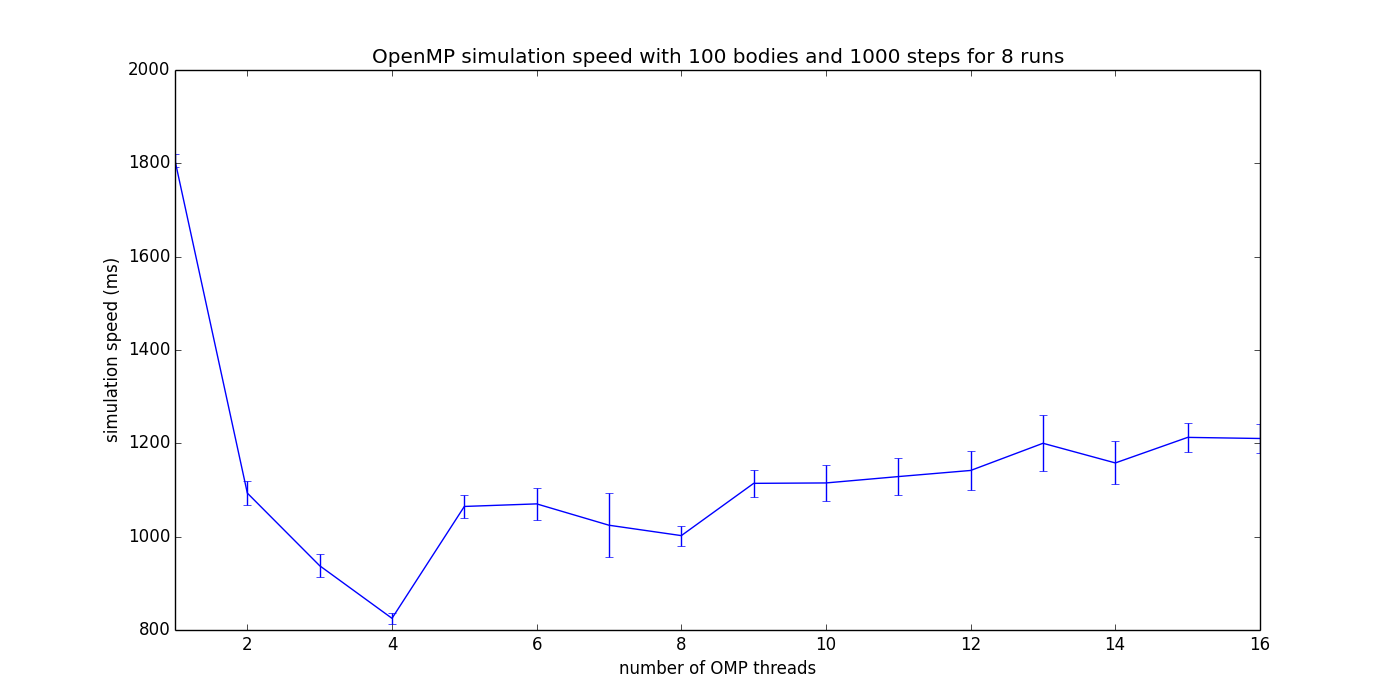
\includegraphics[width=13cm]{img/fig_omp_100b_1000s_8r.png}
\end{frame}

\subsection{Open CL}
\begin{frame}
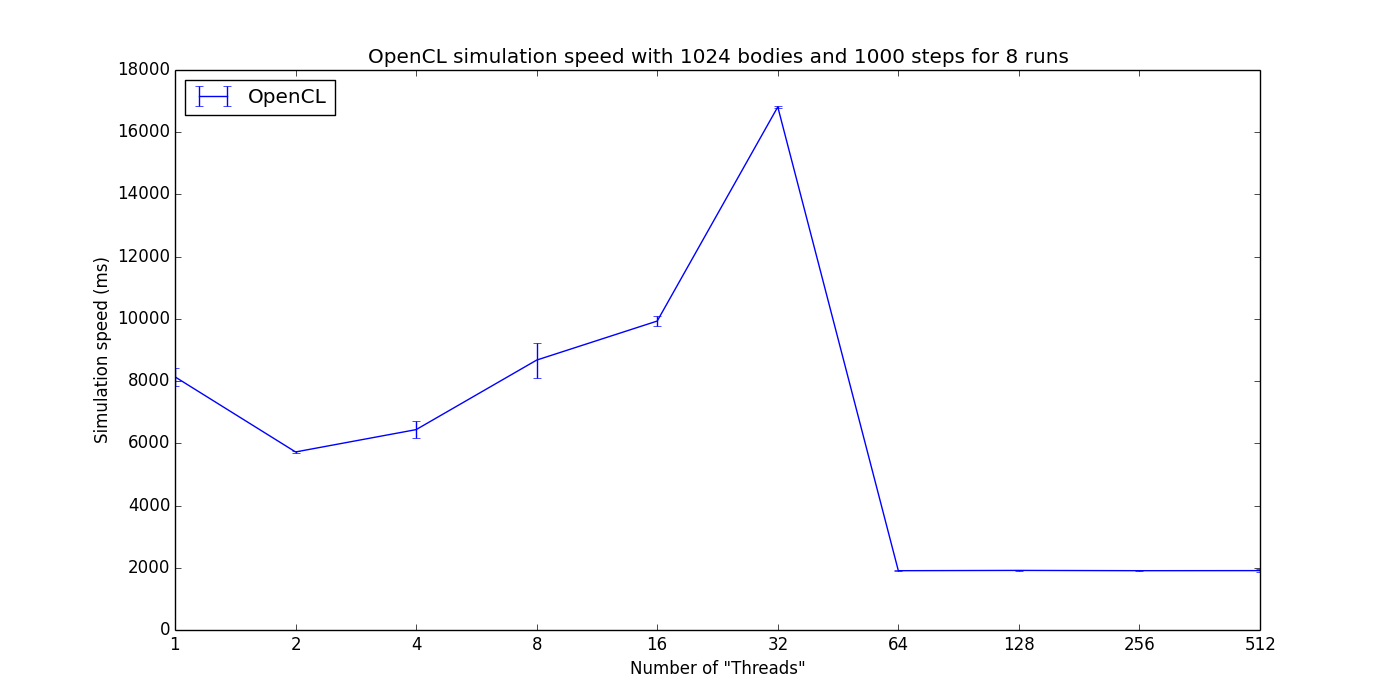
\includegraphics[width=13cm]{img/fig_ocl_1024b_1000s_8r.png}
\end{frame}

\subsection{Vergleich OMP \& OCL}
\begin{frame}
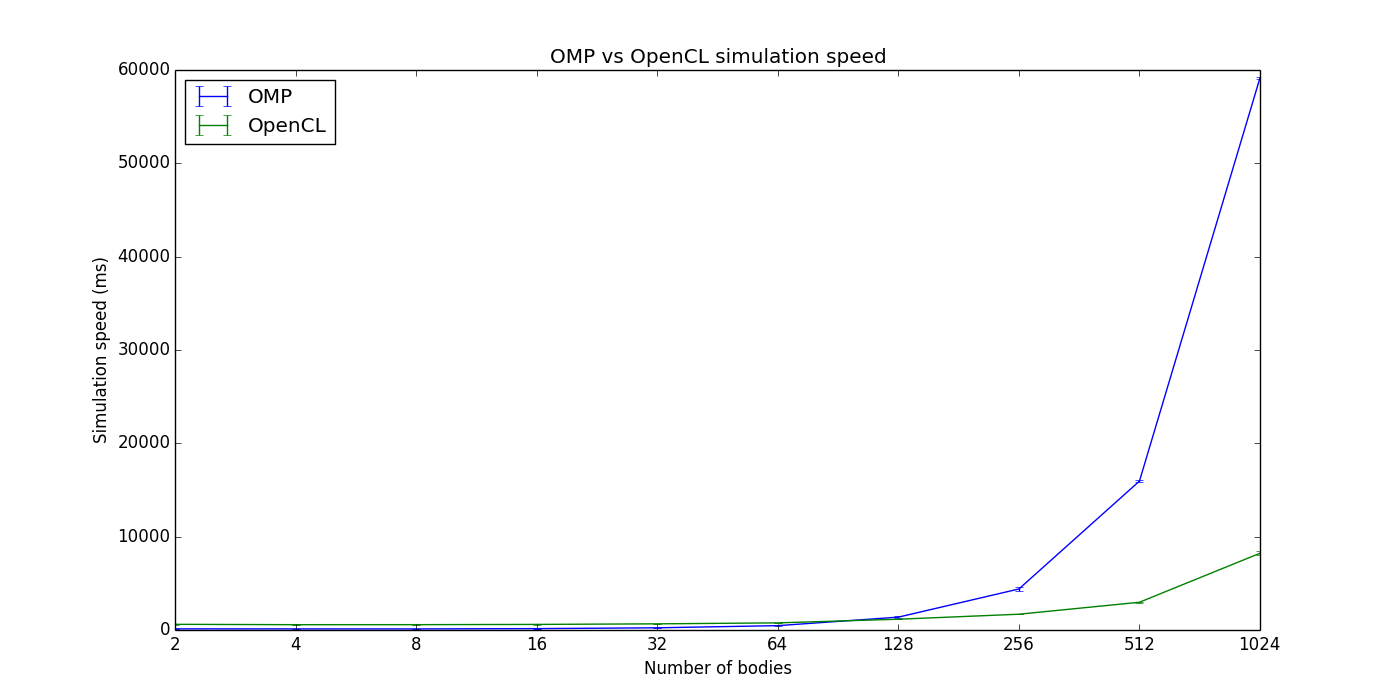
\includegraphics[width=13cm]{img/fig_omp_and_ocl.png}
\end{frame}

\section{Implementierung II}
\subsection{Softwaredesign}
\begin{frame}
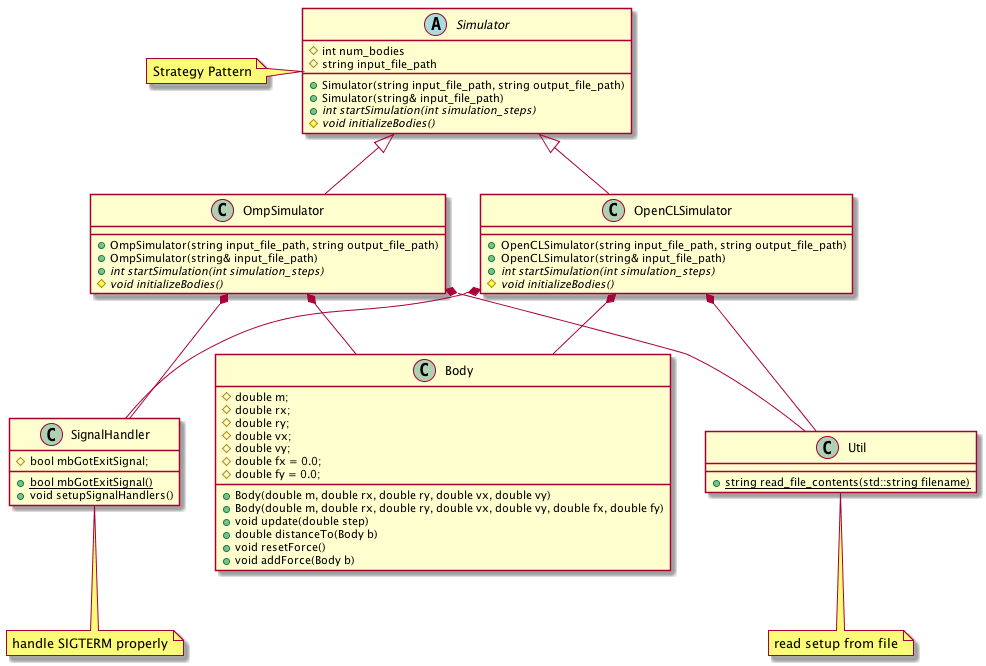
\includegraphics[width=12cm]{img/classes.png}
\end{frame}

\subsection{Visualisierung}
\begin{frame}
\begin{itemize}
  \item konfigurative Initialisierung per Text-File mit Startwerten:
  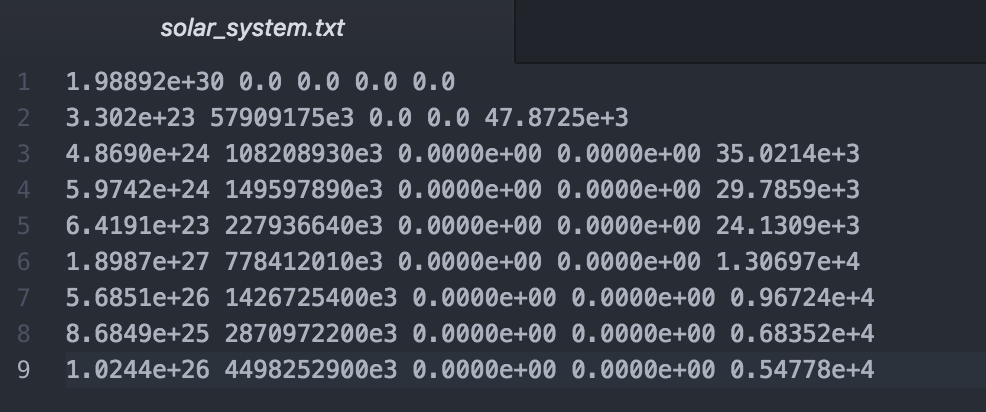
\includegraphics[width=10cm]{img/config_solar.png}
  \begin{itemize}
    \item Konfiguration beinhaltet nur Starteigenschafte für Körper
    \item Wahl des Simulators, Iterationszahl und Logmodus als Programm-Parameter
  \end{itemize}
\end{itemize}
\end{frame}

\subsection{Benchmarks}
\begin{frame}
\begin{itemize}
  \item Simulator loggt Körperkoordinaten in File oder nach stdout
  \item Visualisierung mit Processing-App ließt über Log-Indirektion über Pipe
  \begin{itemize}
    \item $\,\to\,$ Visualisierung in Echtzeit
  \end{itemize}
  \item alternativ auch Loggen auf Platte und Replay der Simulation aus Log-File
  \item Benchmark-Scaffolding mit Python-Skripten
  \begin{itemize}
    \item gutes String- und File-Parsing
    \item einfache Interaktion mit System-Layer (i.e. Anwendung mit dynamischen Parametern starten)
    \item Verfügbarkeit von MatPlotLib
  \end{itemize}
  \item Tests mit GTest (Google)
\end{itemize}
\end{frame}

\section{Vollständigkeit des Belegs}
\subsection{Was bleibt noch zu tun?}
\begin{frame}
ToDo:
\begin{itemize}
  \item valgrind \& helgrind
  \item Doku schreiben
  \item weitere Benchmarks
  \item Test-Coverage erhöhen $\,\to\,$ Refactoring
\end{itemize}
\end{frame}

\section{Demo}
\begin{frame}
  \begin{itemize}
    \item Demo
  \end{itemize}
\end{frame}

\end{document}
